\section{Pushdown Transducers, Automata and Games}
We assume that disjoint sets $\Sigma_\dblI, \Sigma_\dblO$ and $\Gamma$ denote
a (finite) input alphabet, an output alphabet and a stack alphabet, respectively,
and $\Sigma = \Sigma_\dblI \cup \Sigma_\dblO$.
Let $\Com(\Gamma) = \{\pop,\skip\}\cup\{\push(z)\mid z\in \Gamma\}$ be the set of stack commands over $\Gamma$.

\subsection{Pushdown transducers}
\begin{definition}
A {pushdown transducer} (PDT)
over finite alphabets $\Sigma_\dblI$, $\Sigma_\dblO$ and $\Gamma$
is $\calT=(P, p_0, z_0, \Delta)$ where
$P$ is a finite set of states,
$p_0\in P$ is the initial state,
$z_0\in \Gamma$ is the initial stack symbol and
$\Delta: P\times \Sigma_\dblI \times \Gamma \to P\times \Sigma_\dblO \times \Com(\Gamma)$ is a finite set of deterministic transition rules having one of the following forms:
\begin{itemize}
\item $(p, a, z) \rightarrow (q, b, \pop)$ \quad (pop rule)
\item $(p, a, z) \rightarrow (q, b, \skip)$ \quad (skip rule)
\item $(p, a, z) \rightarrow (q, b, \push(z))$ \quad (push rule)
% \item $(p, a, z) \rightarrow (q, \varepsilon, Z)$ \quad (non-$\varepsilon$ rule)
% \item $(p, \varepsilon, z) \rightarrow (q, b, Z)$ \quad ($\varepsilon$ rule)
\end{itemize}
where $p, q\in P$, $a\in\Sigma_\dblI$, $b\in\Sigma_\dblO$ and $z\in\Gamma$.
\end{definition}
\noindent
For a state $p\in P$ and
a finite sequence representing stack contents $u \in \Gamma^*$,
$(p, u)$ is called
a {\em configuration} or {\em instantaneous description (abbreviated as ID)} of PDT $\calT$. Let $\ID_\calT$ denote the set of all IDs of $\calT$.
For $u\in\Gamma^+$ and $\com\in\Com(\Gamma)$, let us define $\upds(u,\com)$
as $\upds(u,\pop)=u(1:)$, $\upds(u,\skip)=u$ and $\upds(u,\push(z'))=z'u$.

For two IDs $(p, u), (q, u')\in \ID_\calT$,
$a\in\Sigma_\dblI$ and $b\in\Sigma_\dblO$,
$((p, u), ab, (q, u'))\in\ \Rightarrow_\calT$,
written as $(p, u) \done_{\calT}^{ab} (q, u')$,
if there exist a rule $(p, a, z) \rightarrow (q, b, \com) \in \Delta$
such that $z=u(0)$ and $u'=\upds(u,\com)$.
If $\calT$ is clear from the context,
we abbreviate
$\done_{\calT}^{ab}$ as $\done^{ab}$.
% If a sequence of IDs $(q_0, w_0), \cdots, (q_n, w_n)\in \ID_\calT$
% and $a_1, \cdots, a_n\in\Sigma_\dblI, b_1, \cdots, b_n\in \Sigma_\dblO$ satisfy $(q_{i-1}, w_{i-1})\done^{a_i, b_i}(q_i, w_i)$ for all $i\in[n]$, we write $(q_0, w_0)\done^{w^\dblI, w^\dblO}(q_n, w_n)$
% where $w^\dblI = a_1 \cdots a_n$ and $w^\dblO = b_1 \cdots b_n$.
% If we emphasize the rule $r$ and the data value $d$,
% we write $\done_d^r$.
% By definition, any ID $(p, \varepsilon)\in\ID_{\calT}$ has
% no successor.
We will use similar abbreviations for the other models defined later.
Note that there is no transition from an ID with empty stack.
We define a run and the language $L(\calT)\subseteq (\Sigma_\dblI \cdot \Sigma_\dblO)^{\omega}$ of PDT $\calT$ as those of
deterministic $0$-TS $(\ID_\calT, (q_0,z_0), \Sigma_\dblI\cdot\Sigma_\dblO, \emptyset, \Rightarrow_\calT, c)$ where $c(s)=2$ for all $s\in\ID_\calT$.
In this paper,
we assume that no run of PDT reaches an ID whose stack is empty.
Let \PDT\ be the class consisting of all PDT.

\begin{example}
\label{ex: PDT}
Let us consider PDT
$\calT = (\{p\},p,z,\Delta)$
over $\{0,1\},\{a,b\}$ and $\{z\}$ where
$\Delta = \{
(p, 0, z) \rightarrow (p, a, \skip),
(p, 1, z) \rightarrow (p, b, \push(z))
\}$
We can see
a pair of sequences $(\rho,w)\in \ID_\calT^\omega\times (\{0,1\}\cdot\{a,b\})^\omega$ where
$\rho=(p,z)(p,z)(p,zz)(p,zz)(p,zzz)(p,zzz)\cdots$
and $w=(0a1b)^\omega$
is a run of $\calT$.
Also, $L(\calT)=(\{0a\}\cup\{1b\})^\omega$.
\end{example}

% Let $(\rho,w)\in \ID_\calT^\omega\times \{a,b\}^\omega$
% be a pair of sequences where
% $\rho=(p,z_0)(p,zz_0)(p,zzz_0)(p,zzzz_0)\cdots$ and $w=aba^\omega$,
% then $(\rho,w)$ is a run of $\calT$.
% Let $\#_a(w), \#_b(w)\in \Natz$ denote the number of $a$, $b$
% appearing in $w\in\{a,b\}^*$, respectively.
% $L(\calT)$ is the set of the sequence $w\in \{a,b\}^\omega$
% that satisfies one of the following conditions:
% (i) $w = t_0 w_0 t_1 w_1\cdots
% \in(\{ab, ba\} \times \{aa, bb\}^*)^\omega$
% where for all $i\geq 0$, $t_i\in \{ab, ba\}$ and
% $w_i\in \{aa, bb\}^*$ such that
% $\#_b(w_i)-\#_a(w_i)=2$.
% (ii) $w = t_0 w_0 t_1 w_1\cdots t_n w_n
% \in(\{ab, ba\}\cdot\{aa, bb\}^*)^*\cdot(\{ab, ba\} \times \{aa, bb\}^\omega)$
% where for all $0\leq i\leq n$, $t_i\in \{ab, ba\}$ and
% $w_i\in \{aa, bb\}^*$ such that
% $\#_b(w_i)-\#_a(w_i)=2$ for $0\leq i< n$ and
% $w_n\in \{aa, bb\}^\omega$ such that
% $\#_a(w')-\#_b(w')\geq 0$
% for all subsequence $w'=w(0:m)$ of $w$ for all $m\in\Natz$.
% \begin{figure}[t]
%   \centering
%   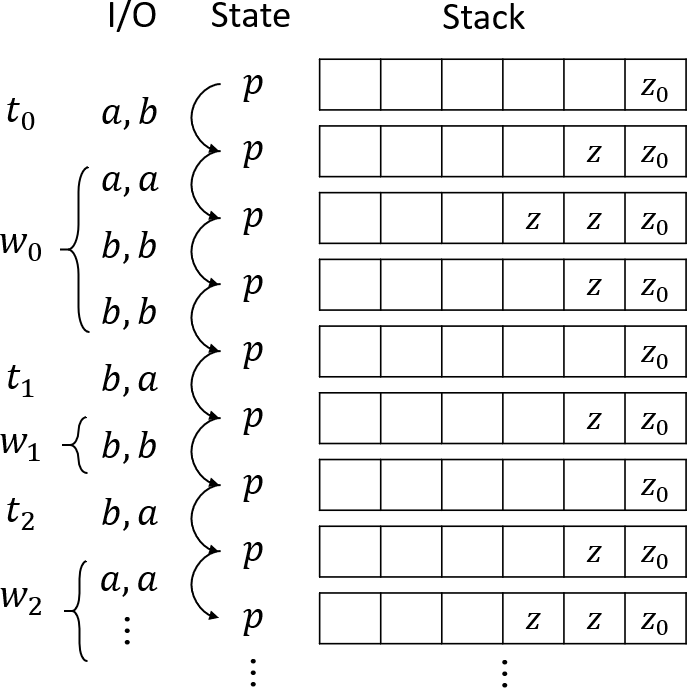
\includegraphics[width=6cm]{PDT.png}
%   \caption{An example of run for a sequence $w = t_0 w_0 t_1 w_1\cdots$.}
%   \label{fig: PDT}
% \end{figure}
% \end{example}

\subsection{Pushdown automata}

\begin{definition}
A nondeterministic {pushdown automata} (NPDA) over finite alphabets $\Sigma_\dblI$, $\Sigma_\dblO$ and $\Gamma$ is $\calA = (Q, Q_\dblI, Q_\dblO, q_0, z_0, \delta, c)$ where
$Q$, $Q_\dblI, Q_\dblO$ are finite sets of states such that $Q=Q_\dblI\cup Q_\dblO$ and $Q_\dblI \cap Q_\dblO = \emptyset$,
$q_0\in Q_\dblI$ is the initial state,
$z_0\in \Gamma$ is the initial stack symbol,
$c: Q \to [n]$ is the coloring function where $n\in \Nat$ is the number of priorities and
$\delta: Q \times \Sigma \times \Gamma \to \scrP(Q \times \Com(\Gamma))$ is a finite set of transition rules having one of the following forms:
\begin{itemize}
\item $(q_\dblX, a_\dblX, z) \rightarrow (q_\overX, \com)$ (input/output rules)
\item $(q_\dblX, \tau, z)\to(q'_\dblX,\com)$ ($\tau$ rules)
\end{itemize}
where $(\dblX, \overX)\in\{(\dblI, \dblO), (\dblO,\dblI)\}$,
$q_\dblX, q'_\dblX\in Q_\dblX, q_\overX\in Q_\overX, a_\dblX\in \Sigma_\dblX$, $z\in \Gamma$ and $\com\in \Com(\Gamma)$.
\end{definition}
We define $\ID_\calA= Q\times \Gamma^*$ and
the transition relation $\vdash_\calA\subseteq \ID_\calA\times (\Sigma\cup\{\tau\})\times \ID_\calA$ as
$((q,u),a,(q',u'))\in\ \vdash_\calA$ iff there exist a rule $(q, a, z) \rightarrow (q', \com) \in \delta$ and a sequence $u\in \Gamma^*$ such that $z=u(0)$ and $u'=\upds(u,\com)$.
We write $(q,u)\vdash^a_\calA(q',u')$ iff
$((q,u),a,(q',u'))\in\ \vdash_\calA$.
We define a run and the language $L(\calA)$ of $\calA$ as those of TS $\calS_\calA=(\ID_\calA, (q_0,z_0),\Sigma, \{\tau\},\vdash_\calA,c')$
where $c'((q,u))= c(q)$ for every $(q,u)\in\ID_\calA$.
% We call a PDA $\calA=(P, p_0, z_0, \delta, c)$ deterministic if $|\delta(p,a,z)|\leq 1$ for all $p\in Q, a\in\Sigma$ and $z\in\Gamma$.
We call a PDA $\calA$ deterministic if $\calS_\calA$ is deterministic.
We call $\calA$ an $m$-NPDA (or $m$-DPDA when $\calA$ is deterministic)
if $\calS_\calA$ is an $m$-TS.
We abbreviate $0$-NPDA ($0$-DPDA) as NPDA (DPDA).
% nondeterministic if the language is defined as $L_N(\calS_\calA)$,
% universal if the language is defined as $L_U(\calS_\calA)$.
Let $\DPDA$ and $\NPDA$ be the classes of DPDA and NPDA, respectively.

\begin{example}
\label{ex: PDA}
Let us consider DPDA
$\calA = (\{q,q',q_a,q_b\},\{q,q'\},\{q_a,q_b\},q,z,\delta,c)$
over $\{0,1\},\{a,b\}$ and $\{z\}$ where
$c(q')=1$, $c(s)=2$ for $s=q,q_a,q_b$ and
$\delta$ is defined as in Fig. \ref{fig: PDA}.
% $\delta = \{
% (q, 0, z) \rightarrow (q_a, \skip),
% (q, 1, z) \rightarrow (q_b, \skip),
% (q_a, a, z) \rightarrow (q, \push(z)),
% (q_b, b, z) \rightarrow (q, \push(z)),
% (q_a, b, z) \rightarrow (q', \pop),
% (q_b, a, z) \rightarrow (q', \pop),
% (q', 0, z) \rightarrow (q_a, \skip),
% (q', 1, z) \rightarrow (q_b, \skip)
% \}$.
We can see
a pair of sequences $(\rho,w)\in \ID_\calT^\omega\times (\{0,1\}\cdot\{a,b\})^\omega$ in Example \ref{ex: PDT},
where $\rho=(q,z)(q,z)(q,zz)(q,zz)(q,zzz)(q,zzz)\cdots$
and $w=(0a1b)^\omega$,
is also a run of $\calA$.
However, $w_1=(0a1a)^\omega$ and $w_2=0b(0a1b)^\omega$
are not in $L(\calA)$ because
the run $(\rho_1,w_1)$ visits $q'$ infinitely and
the input sequence $w_2$ forces a stack of $\calA$ empty
by reading $0b$ first.
We call $0a$ and $1b$ push subsequences and $0b$ and $1a$ pop subsequences.
For a sequence $w\in(\{0,1\}\cdot\{a,b\})^\infty$,
let $\#_{push}(w)$ and $\#_{pop}(w)$ be the number of
push and pop subsequences appearing in $w$, respectively.
We can check
$L(\calA)=\{w\in(\{0,1\}\cdot\{a,b\})^\omega\mid
\#_{pop}(w)$ is finite and
$\#_{push}(w')-\#_{pop}(w')\geq 0$
for every subsequence $w'=w(0:m)$ of $w$ for all $m\in\Natz\}$.
For PDT $\calT$ defined in Example \ref{ex: PDT},
we know $L(\calT)\subseteq L(\calA)$
because $L(\calT)=(\{0a\}\cup\{1b\})^\omega$ contains no sequence that includes a pop subsequence.
\end{example}
\begin{figure}[t]
  \centering
  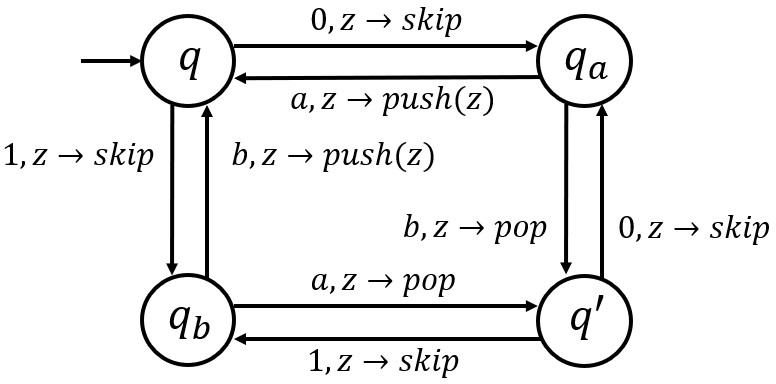
\includegraphics[width=8cm]{PDA.png}
  \caption{States and transitions of $\calA$.
  (A label $a,b \to c$ from $q$ to $q'$ means
  $(q,a,b)\to(q',c)\in\delta$.)}
  \label{fig: PDA}
\end{figure}

The following lemma states that
the class of languages recognized by $m$-DPDA and $0$-DPDA are the same
for a fixed $m$.
\begin{lemma}
\label{lem: ef}
For a given $m$-DPDA $\calA$,
we can construct a $0$-DPDA $\calA'$ such that
$L(\calA)=L(\calA')$
\end{lemma}\
{\bf Proof sketch}\quad
We define the stack alphabet $\Gamma'$ of $\calA'$ as $\Gamma'=\Gamma^m$.
We can simulate $m$-steps with consecutive push rules (or pop rules) of $\calA$
by a single step with a push (or pop) rule of $\calA'$.

% \begin{example}
% \label{ex: PDA}
% Let us consider DPDA
% $\calA = (\{q_0,q_\bot,q_\dblI,q_\dblO\}, \{q_0,q_\dblI\}, \{q_\bot,q_\dblO\},q_0,z_0,\delta,c)$
% over $\{0,1\},\{a,b\}$ and $\{z_0,z\}$ where
% $c(q_\bot)=1$, $c(p)=2$ for $p = q_0,q_\dblI,q_\dblO$ and
% $\delta$ is defined as Fig. \ref{fig: PDA},
% in detail,
% $\delta = \{
% (p, x, z_0) \rightarrow (q_\bot, \push(z))\mid
% p\in\{q_0,q_\dblI\}, x\in\{a,b\}\}\cup
% \{(q_\bot, x, z) \rightarrow (q_\dblI, \push(z))\mid x\in\{a,b\}\}\cup
% \{(p, a, z) \rightarrow (p', \push(z)),
% (p, b, z) \rightarrow (p', \pop)\mid
% (p,p')\in\{(q_\dblI,q_\dblO), (q_\dblO,q_\dblI)\}\}$.
% For example, we can check the sequence
% $(\rho,w)\in \ID_\calT^\omega\times \{a,b\}^\omega$
% where $\rho =(q_0,z_0)(q_\bot,zz_0)(q_\dblI,zzz_0)(q_\dblO,zzzz_0)
% (q_\dblI,zzzzz_0)(q_\dblO,zzzzzz_0)\cdots$
% and $w=aba^\omega$ is a run of $\calA$.
% Because $q_\bot$ appears only one times in $\rho$,
% $w\in L(\calA)$ holds.
%
% $L(\calA)$ is the set of the sequence $w\in \{a,b\}^\omega$
% that satisfies one of the following conditions:
% (i) $w = t_0 w_0 t_1 w_1\cdots
% \in(\{ab,ba\} \times \{a,b\}^*)^\omega$
% where for all $i\geq 0$, $t_i\in \{ab, ba\}$ and
% $w_i\in \{a,b\}^*$ such that
% $\#_b(w_i)-\#_a(w_i)=2$.
% (ii) $w = t_0 w_0 t_1 w_1\cdots t_n w_n
% \in(\{ab,ba\} \times \{a,b\}^*)^*\cdot(\{ab,ba\} \times \{a,b\}^\omega)$
% where for all $0\leq i\leq n$, $t_i\in \{ab, ba\}$ and
% $w_i\in \{a,b\}^*$ such that
% $\#_b(w_i)-\#_a(w_i)=2$ for $0\leq i< n$ and
% $w_n\in \{a,b\}^\omega$ such that
% $\#_a(w')-\#_b(w')\geq 0$
% for all subsequence $w'=w(0:m)$ of $w$ for all $m\in\Natz$.
% To compare with PDT $\calT$ defined in Example \ref{ex: PDT},
% we can check $L(\calT)\subseteq L(\calA)$.
% \end{example}
% \begin{figure}[t]
%   \centering
%   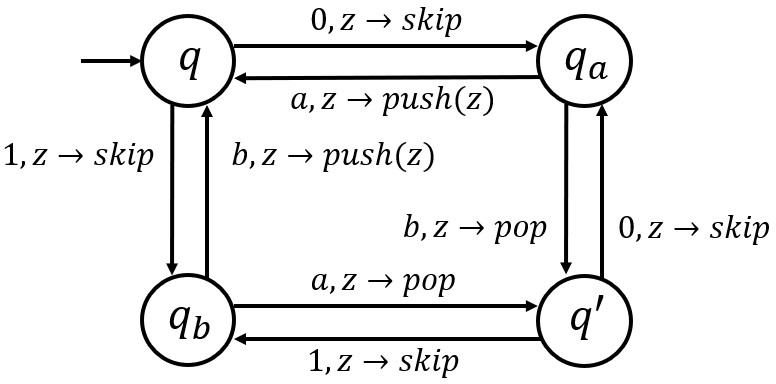
\includegraphics[width=10cm]{PDA.png}
%   \caption{States and transitions of $\calA$.
%   (A label $a,b \to c$ from $q$ to $q'$ means
%   $(q,a,b)\to(q',c)\in\delta$.)}
%   \label{fig: PDA}
% \end{figure}

\subsection{Pushdown games}

\begin{definition}
A {pushdown game} of DPDA $\calA = (Q, Q_\dblI, Q_\dblO, q_0, z_0, \delta, c)$ over $\Sigma_\dblI, \Sigma_\dblO$ and $\Gamma$ is $\calG_\calA = (V, V_\dblI, V_\dblO, E, C)$ where
$V = Q\times\Gamma^*$ is the set of vertices with $V_\dblI = Q_\dblI\times\Gamma^*, V_\dblO = Q_\dblO\times\Gamma^*$, $E\subseteq V\times V$ is the set of edges defined as $E = \{(v,v') \mid v \vdash^a v' \text{for some $a\in \Sigma_\dblI\cup\Sigma_\dblO$}\}$
and $C: V \to [n]$ is the coloring function such that
$C((q,u)) = c(q)$ for all $(q,u)\in V$.
\end{definition}

The game starts with $(q_0,z_0)\in V_\dblI$.
When the current vertex is $v\in V_\dblI$,
Player II chooses a successor $v'\in V_\dblO$ of $v$ as the next vertex.
When the current vertex is $v\in V_\dblO$,
Player I chooses a successor $v'\in V_\dblI$ of $v$.
Formally, a finite or infinite sequence $\rho\in V^\infty$ is
\emph{valid} if
$\rho(0)=(q_0,z_0)$ and
$(\rho(i-1), \rho(i))\in E$ for every $i\geq 1$.
A \emph{play} of $\calG_\calA$ is an infinite and valid sequence $\rho\in V^\omega$.
Let $\PL$ be the set of plays.
A play $\rho\in \PL$ is \emph{winning} for Player I iff
$\min\{m\in[n] \mid $ there exist an infinite
number of $i\geq 0$ such that $c(\rho(i)) = m\}$ is even.

Since $\calA$ is deterministic,
the following lemma holds.
\begin{lemma}
\label{lem: cor}
Let $f_1: \PL\to(Q\times\Com(\Gamma))^\omega$ and
$f_2: \PL\to\Sigma^\omega$ be the functions defined as follows.
For every play
$\rho=(q_0,u_0)(q_1,u_1)\cdots\in \PL$ of $\calG_\calA$,
\begin{itemize}
\item $f_1(\rho)=(q_0,\com_0)(q_1,\com_1)\cdots\in (Q\times\Com)^\omega$ where
$u_{i+1} = \upds(u_{i},\com_i)$
for all $i\geq 0$ and
\item $f_2(\rho)=w$ where $\rho(i)\vdash^{w(i)} \rho(i+1)$
for all $i\geq 0$.
\end{itemize}
Then, $f_1$ and $f_2$ are well-defined and both of $f_1$ and $f_2$ are injections.
\end{lemma}
% {\bf Proof.}\quad
% We show both of sequences
% $\pi=(q_0,\com_0)(q_1,\com_1)\cdots\in (Q\times\Com)^\omega$
% and $w\in\Sigma^\omega$
% determinine a play
% $\rho=(q_0,u_0)(q_1,u_1)\cdots\in V^\omega$ uniquely.
% From $\pi$, we let $u\in (\Gamma^*)^\omega$ such that
% $u_0 = z_0$ and $u_{i+1} = \upds(u_{i},\com_i)$
% for all $i\geq 0$.
% Then a play
% $\rho=(q_0,u_0)(q_1,u_1)\cdots\in V^\omega$
% is determined uniquely.
% From $w$, we let a sequence $\rho\in V^\omega$
% such that there exists a run $(\rho,w)$ of $\calA$.
% Because $\calA$ is deterministic,
% $\rho$ is determined uniquely.
% \par\medskip\noindent
It is proved in \cite{Wa96} that
we can construct a PDT $\calT$
that gives a winning strategy of $\calG_\calA$,
that is, $L(\calT) = \{ f_1(\rho) \mid
\rho$ is winning for Player I $\}$.
% [Walukiewucz, 2001] proved that
% we can construct an PDT $\calT$ such that
% $L(\calT)$ equals to the set of all sequences $\pi\in (Q\times\Com)^\omega$ whose corresponding play is winning.
\begin{theorem}{\cite{Wa96}}
\label{the: wal}
If player I has a winning strategy of $\calG_\calA$,
we can construct a PDT $\calT$ over $Q_\dblI\times\Com(\Gamma), Q_\dblO\times\Com(\Gamma)$ and a stack alphabet $\Gamma'$ that gives a winning strategy of $\calG_\calA$.
That is, $\rho\in \PL$ is winning for Player I if $f_1(\rho)\in L(\calT)$.
\end{theorem}

By Lemma \ref{lem: cor},
a winning strategy can be also given as
the set of sequences $w\in\Sigma^\omega$
such that the play $\rho$ is winning where $f_2(\rho)=w$.
Thus, we can obtain the following lemma
in a similar way to Theorem \ref{the: wal}.
\begin{corollary}
\label{col: 2}
If player I has a winning strategy of $\calG_\calA$,
we can construct a PDT $\calT$ over $\Sigma_\dblI, \Sigma_\dblO$ and $\Gamma'$ that gives a winning strategy of $\calG_\calA$.
That is, $\rho\in \PL$ is winning for Player I if $f_2(\rho)\in L(\calT)$.
\end{corollary}
